\chapter{Vectors and Geometry of Space}

\section{Three-Dimensional Coordinate Systems}

\subsection*{3D Space}
The direction of the $z$-axis is determined by the \textbf{right-hand rule}.
if you curl the fingers of your right hand around the $z$-axis, in the clockwise direction
from the $x$-axis to the $y$-axis, your thumb points in the direction of the $z$-axis.

The Cartesian product $\mathbb{R}\times\mathbb{R}\times\mathbb{R}=
    \{x,y,z\} | x,y,z \in \mathbb{R}$ is the set of all ordered triples of real numbers
and is denoted by $\mathbb{R}^3$.

\subsection*{Surfaces}
In three-dimensions, an equation in $x,y,z$ represents a \emph{surface} in $\mathbb{R}^3$.

\subsection*{Example}
What surfaces in $\mathbb{R}^3$ are represented by the following equations?
\begin{enumerate}[(a)]
    \item $z=3$
    \item $y=5$
\end{enumerate}
\subsection*{Solution}
(a) $z=3$ represents the set $\{x,y,z | z=3\}$, which all the points in
$\mathbb{R}^3$ whose $z$-coordinate is 3. This is a horizontal plane parallel
to the $xy$-plane and three units above it. \\
(b) $y=5$ represents a vertical plane parallel to the $xz$-plane and five units
to the right of it.

\textbf{Distance Formula in Three Dimensions} \\
The distance $|P_1P_2|$ between the points $P_1(x_1,y_1,z_1)$ and $P_2(x_2,y_2,z_2)$ is
$$|P_1P_2|=\sqrt{(x_2-x_1)^2+(y_2-y_1)^2+(z_2-z_1)^2}$$

\textbf{Equation of a Sphere} \\
An equation of a sphere with center $C(h,k,l)$ and radius $r$ is
$$ (x-h)^2+(y-k)^2+(z-l)^2=r^2 $$
If the center is the origin $O$, then the equation is
$$ x^2+y^2+z^2=r^2 $$

\subsection*{Example}
What region in $\mathbb{R}^3$ is represents by the following inequalities?
$$1\leq x^2+y^2+z^2\leq 4 \qquad z\leq 0$$
\subsection*{Solution}
The inequalities can be rewritten as
$$1\leq \sqrt{x^2+y^2+z^2}\leq 2$$
so they represent the points $(x,y,z)$ whose distance from the origin is at least 1 and at most 2.
\begin{center}
    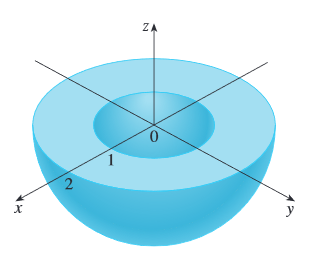
\includegraphics[scale=0.7]{example13-1}
\end{center}

\section{Vectors}

\subsection*{Combining Vectors}
\textbf{Definition of Vector Addition} \\
If \textbf{u} and \textbf{v} are vectors positioned
so the intial point of \textbf{v} is at the terminal point of \textbf{u}, then
the sum \textbf{u + v} is the vector from the initial point of \textbf{u}
to the terminal point of \textbf{v}.
\begin{center}
    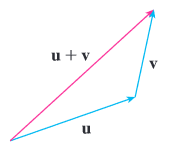
\includegraphics[scale=0.7]{example13-2-1}
\end{center}

\textbf{Definition of Scalar Multiplication} \\
If $c$ is scalar and \textbf{v} is a vector, then the \textbf{scalar multiple}
$c\mathbf{v}$ is the vector whose length is $|c|$ times the length of
\textbf{v} and whose direction is the same as \textbf{v} if $c>0$ and
is opposite to \textbf{v} if $c<0$.
\begin{center}
    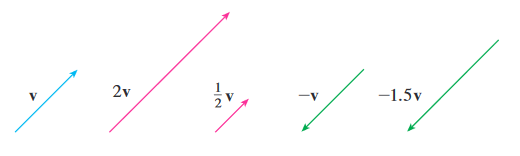
\includegraphics[scale=0.7]{example13-2-2}
\end{center}

\subsection*{Components}
The \textbf{components} of vector \textbf{a} are written as
$$\mathbf{a}=\ev{a_1,a_2} \qquad \mathbf{a}=\ev{a_1,a_2,a_3}$$

\subsection*{Example}
Find the vector represented by the directed line segment with initial
point $A(2,-3,4)$ and terminal point $B(-2,1,1)$.

\subsection*{Solution}
$$\mathbf{a}=\ev{x_2-x_1,y_2-y_1,z_2-z_1}$$
$$\mathbf{a}=\ev{-2-2,1-(-3),1-4}=\ev{-4,4,-3}$$

\subsection*{Example}
If \textbf{a}=$\ev{4,0,3}$, find $|\textbf{a}|$.

\subsection*{Solution}
$$|\textbf{a}|=\sqrt{4^2+0^2+3^2}=\sqrt{25}=5$$

\subsection*{Properties of Vectors}
If \textbf{a}, \textbf{b}, and \textbf{c} are vectors in $V_n$ and $c$ and $d$ are scalars
\begin{multicols}{2}
    \begin{enumerate}
        \item $\textbf{a+b=b+a}$
        \item $\textbf{a+(b+c)=(a+b)+c}$
        \item $\textbf{a+0=a}$
        \item $\textbf{a+(-a)=0}$
        \item $c\textbf{(a+b)}=c\textbf{a}+c\textbf{b}$
        \item $(c+d)\textbf{a}=c\textbf{a}+d\textbf{a}$
        \item $(cd)\textbf{a}=c(d\textbf{a})$
        \item $1\textbf{a}=\textbf{a}$
    \end{enumerate}
\end{multicols}

\textbf{Standard Basis Vectors}
$$ \textbf{i}=\ev{1,0,0} \qquad \textbf{j}=\ev{0,1,0} \qquad \textbf{k}=\ev{0,0,1} $$

\subsection*{Example}
Find the unit vector in the direction of the vector $2\textbf{i}-\textbf{k}-2\textbf{k}$.

\subsection*{Solution}
The given vector has length
$$|2\textbf{i}-\textbf{k}-2\textbf{k}|=\sqrt{2^2+(-1)^2+(-2)^2}=\sqrt{9}=3$$
and by the equation $\textbf{u}=\cfrac{1}{|\textbf{a}|}\textbf{a}=\cfrac{\textbf{a}}{|\textbf{a}|}$,
the unit vector is
$$\frac{1}{3}(2\textbf{i}-\textbf{j}-2\textbf{k})=\frac{2}{3}\textbf{i}-
    \frac{1}{3}\textbf{j}-\frac{2}{3}\textbf{k}$$

\section{The Dot Product}

\subsection*{Definition}
If $\textbf{a}=\ev{a_1,a_2,a_3}$ and $\textbf{b}=\ev{b_1,b_2,b_3}$, then the
\textbf{dot product} of \textbf{a} and \textbf{b} is
$$\mathbf{a\cdot b}=a_1 b_1+a_2 b_2+a_3 b_3$$

\subsection*{Properties of the Dot Product}
If \textbf{a}, \textbf{b}, and \textbf{c} are vectors in $V_3$ and $c$ is scalar
\begin{multicols}{2}
    \begin{enumerate}
        \item $\mathbf{a\cdot a=|a|^2}$
        \item $\mathbf{a\cdot b=b\cdot a}$
        \item $\mathbf{a\cdot (b\cdot c)=a\cdot b+a\cdot c}$
        \item $(c\mathbf{a})\cdot\mathbf{b}=c(\mathbf{a\cdot b})=\mathbf{a}\cdot(c\mathbf{b})$
        \item $\mathbf{0\cdot a}=0$
        \item []
    \end{enumerate}
\end{multicols}

\subsection*{Theorem}
If $\theta$ is the angle between the vectors \textbf{a} and \textbf{b}, then
$$\mathbf{a\cdot b} = \mathbf{|a||b|}\:cos\:\theta$$

Two nonzero vectors are \textbf{perpendicular} or \textbf{orthogonal} if the angle
between then is $\theta=\pi/2$. The dot product gives
$$\mathbf{a\cdot b}=\mathbf{|a||b|}\:cos(\pi/2)=0$$
Two vectors \textbf{a} and \textbf{b} are orthogonal if and only if $\mathbf{a\cdot b}=0$.

\subsection*{Projections}
Scalar projection of \textbf{b} onto \textbf{a}: $\qquad comp_a\textbf{b}=
    \mathbf{\cfrac{a\cdot b}{|a|}}$ \\
Vector projection of \textbf{b} onto \textbf{a}: $\qquad proj_a\textbf{b}=
    \mathbf{\left(\cfrac{a\cdot b}{|a|}\right)\cfrac{a}{|a|}}=\mathbf{\cfrac{a\cdot b}{|a|^2}a}$

\subsection*{Example}
Find the scalar projection and vector projection of $\textbf{b}=\ev{1,1,2}$ onto
$\textbf{a}=\ev{-2,3,1}$.

\subsection*{Solution}
Since $|\textbf{a}|=\sqrt{(-2)^2+3^2+1^2}=\sqrt{14}$, the scalar projection of \textbf{b}
onto \textbf{a} is:
$$comp_a\textbf{b}=\mathbf{\frac{a\cdot b}{|a|}}=\frac{(-2)(1)+3(1)+1(2)}{\sqrt{14}}=\frac{3}{\sqrt{14}}$$
The vector projection is this scalar projection times the unit vector in the direction of \textbf{a}:
$$proj_a\textbf{b}=\frac{3}{\sqrt{14}}\mathbf{\frac{a}{|a|}}=\frac{3}{14}\textbf{a}=
    \ev{-\frac{3}{7},\frac{9}{14},\frac{3}{14}}$$

\section{The Cross Product}

\subsection*{Definition}
If $\textbf{a}=\ev{a_1,a_2,a_3}$ and $\textbf{b}=\ev{b_1,b_2,b_3}$, then the
\textbf{cross product} of \textbf{a} and \textbf{b} is the vector
$$\mathbf{a \times b}=\ev{a_2b_3-a_3b_2,a_3b_1-a_1b_3,a_1b_2-a_2b_1}$$
This Definition can be rewritten using second-order determinants and the standard
basis vectors \textbf{i, j,} and \textbf{k}
$$\mathbf{a\times b}=\
    \begin{vmatrix}
        \textbf{i} & \textbf{j} & \textbf{k} \\
        a_1        & a_2        & a_3        \\
        b_1        & b_2        & b_3
    \end{vmatrix}$$


\subsection*{Example}
If $\textbf{a}=\ev{1,3,4}$ and $\textbf{b}=\ev{2,7,-5}$, then
\begin{align*}
    \mathbf{a\times b} & =\
    \begin{vmatrix}
        \textbf{i} & \textbf{j} & \textbf{k} \\
        1          & 3          & 4          \\
        2          & 7          & -5
    \end{vmatrix}                                                                                                               \\
                       & =\begin{vmatrix}
        3 & 4  \\
        7 & -5
    \end{vmatrix}\textbf{i} - \begin{vmatrix}
        1 & 4  \\
        2 & -5
    \end{vmatrix}\textbf{j} + \begin{vmatrix}
        1 & 3 \\
        2 & 7
    \end{vmatrix}\textbf{k} \\
                       & =(-15-28)\textbf{i}-(-5-8)\textbf{j}+(7-6)\textbf{k}=-43\textbf{i}+13\textbf{j}+\textbf{k}
\end{align*}


\subsection*{Theorem}
The vector $\mathbf{a\times b}$ is orthogonal to both \textbf{a} and \textbf{b}.

\subsubsection*{Proof} $\mathbf{(a\times b)\cdot b}=0$. Therefore $\mathbf{a\times b}$
is orthogonal to both \textbf{a} and \textbf{b}.

\subsection*{Theorem}
If $\theta$ is the angle between \textbf{a} and \textbf{b} (so $0\leq \theta \leq \pi$), then
$$|\mathbf{a\times b}|=\mathbf{|a||b|}\:sin\:\theta$$

\subsection*{Corollary}
Two nonzero vectors \textbf{a} and \textbf{b} are parallel if and only if
$$\mathbf{a\times b=0}$$

\subsection*{Example}
Find the vector perpendicular to the plane that passes through the points $P(1,4,6)$,
$Q(-2,5,-1)$, and $R(1,-1,1)$.

\subsection*{Solution}
\begin{enumerate}
    \item[] $\overrightarrow{PQ}=(-2-1)\textbf{i}+(5-4)\textbf{j}+(-1-6)\textbf{k}=\mathbf{-3i+j-7k}$
    \item[] $\overrightarrow{PR}=(1-1)\textbf{i}+(-1-4)\textbf{j}+(1-6)\textbf{k}=\mathbf{-5j-5k}$
\end{enumerate}
We compute the cross product of these vectors:
$$\overrightarrow{PQ}\times \overrightarrow{PR}=\begin{vmatrix}
        \textbf{i} & \textbf{j} & \textbf{k} \\
        -3         & 1          & -7         \\
        0          & -5         & -5
    \end{vmatrix}=-40\textbf{i}-15\textbf{j}+15\textbf{k}$$

\subsection*{Properties of the Cross Product}
If \textbf{a, b,} and \textbf{c} are vectors and $c$ is a scalar, then
\begin{enumerate}
    \item $\mathbf{a\times b=-b\times a}$
    \item $(c\textbf{a})\times \textbf{b}=c(\mathbf{a\times b})=\textbf{a}\times(c\textbf{b})$
    \item $\mathbf{a\times (b+c)=a\times b+a\times c}$
    \item $\mathbf{(a+b)\times c=a\times c+b\times c}$
    \item $\mathbf{a\cdot (b\times c)=(a\times b)\cdot c}$
    \item $\mathbf{a\times (b\times c)=(a\cdot c)b-(a\cdot b)c}$
\end{enumerate}

\subsection*{Triple Products}
The volume of the parallelepiped determined by the vectors \textbf{a, b,} and \textbf{c}
is the magnitude of their scalar triple product:
$$V=|\mathbf{a\cdot (b\times c)}|=\begin{vmatrix}
        a_1 & a_2 & a_3 \\
        b_1 & b_2 & b_3 \\
        c_1 & c_2 & c_3
    \end{vmatrix}$$
When the volume is 0, the vectors lie in the same plane and are \textbf{coplanar}.

\section{Equations of Lines and Planes}

\subsection*{Lines}

$$\textbf{r}=\textbf{r}_0|t\textbf{v}$$
is the \textbf{vector equation} of $L$. Each value of the \textbf{parameter} $t$ gives
the position vector \textbf{r} of a point on $L$. We can also write $\textbf{r}=\ev{x,y,z}$
and $\textbf{r}_0=\ev{x_0,y_0,z_0}$, so the vector equation becomes
$$\ev{x,y,z}=\ev{x_0+ta,y_0+tb,z_0+tc}$$

\subsection*{Example}
Find a vector equation and parametric equations for the line that passes through the point
$(5,1,3)$ and is parallel to the vector $\textbf{i}+4\textbf{j}-2\textbf{k}$.

\subsection*{Solution}
Here $\textbf{r}_0=\ev{5,1,3}=5\textbf{i}+\textbf{j}+3\textbf{k}$ and
$\textbf{v}=\textbf{i}+4\textbf{j}-2\textbf{k}$, so the vector equation becomes
\begin{enumerate}
    \item[] $\textbf{r}=(5\textbf{i}+\textbf{j}+3\textbf{k})+t(\textbf{i}+4\textbf{j}-2\textbf{k})$
    \item[] $\textbf{r}=(5+t)\textbf{i}+(1+4t)\textbf{j}+(3-2t)\textbf{k}$
\end{enumerate}
Parametric equations are
$$x=5+t \qquad y=1+4t \qquad z=3-2t$$

\subsection*{Planes}

$$\textbf{n}\cdot (\textbf{r}-\textbf{r}_0=0)$$
which can be rewritten as
$$\mathbf{n\cdot r}=\textbf{n}\cdot \textbf{r}_0$$
Either of the two equations are the \textbf{vector equation of the plane}.

A \textbf{scalar equation of the plane} through point $P_0(x_0,y_0,z_0)$ with normal
vector $\textbf{n}=\ev{a,b,c}$ is
$$a(x-x_0)+b(y-y_0)+c(z-z_0)=0$$
which can be rewritten as
$$ax+by+cz+d=0$$
where $d=-(ax_0+by_0+cz_0)$.

\subsection*{Example}
Find an equation of the plane that passes through the points $P(1,3,2)$, \newline
$Q(3,-1,6)$, and $R(5,2,0)$.

\subsection*{Solution}
The vectors \textbf{a} and \textbf{b} corresponding to $\overrightarrow{PQ}$ and
$\overrightarrow{PR}$ are
$$\textbf{a}=\ev{2,-4,4} \qquad \textbf{b}=\ev{4,-1,-2}$$
Since both \textbf{a} and \textbf{b} lie in the plane, their cross product $\mathbf{a\times b}$
is orthogonal to the plane and can be taken as the normal vector. Thus
$$\mathbf{n=a\times b}=\begin{vmatrix}
        \textbf{i} & \textbf{j} & \textbf{k} \\
        2          & -4         & 4          \\
        4          & -1         & -2
    \end{vmatrix}=12\textbf{i}+20\textbf{j}+14\textbf{k}$$
With the point $P(1,3,2)$ and the normal vector \textbf{n}, an equation of the plane is
$$12(x-1)+20(y-3)+14(z-2)=0$$
or
$$6x+10y+7z=50$$

\subsection*{Distances}
The formula for the distance $D$ can be written as
$$D=\frac{|ax_1+by_1+cz_1+d|}{\sqrt{a^2+b^2+c^2}}$$

\subsection*{Example}
Find the distance between the parallel planes $10x+2y-2z-5$ and $5x+y-z=1$

\subsection*{Solution}
The planes are parallel because their normal vectors $\ev{10,2,-2}$ and
$\ev{5,1,-1}$ are parallel. To find the distance between the planes, we choose
any point on one plane and calculate its distance to the other plane. If we
plug in $y=z=0$ into the first equation, we get $10x=5$ and so $(\frac{1}{2},0,0)$
is a point in the plane.
$$D=\frac{|5(\frac{1}{2})+1(0)-1(0)-1|}{\sqrt{5^2+1^2+(-1)^2}}=\frac{\frac{3}{2}}{3\sqrt{3}}
    =\frac{\sqrt{3}}{6}$$

\section{Cylinders and Quadric Surfaces}

\subsection*{Cylinders}
A \textbf{cylinder} is a surface that consists of all lines that are parallel to a
given line and pass through a given plane curve.

\subsection*{Quadric Surfaces}
A \textbf{quadric surface} is the graph of a second-degree equation in three variables
$x$, $y$, and $z$. The most general such equation is
$$Ax^2+By^2+Cz^2+Dxy+Eyz+Fxz+Gx+Hy+Iz+J=0$$
where $A, B, C, \dots , J$ are constants, but by translation and rotation it can be
brought into one of the two standard forms
$$Ax^2+By^2+Cz^2+J=0 \qquad Ax^2+By^2+Iz=0$$

\subsection*{Graphs of Quadric Surfaces}
\begin{center}
    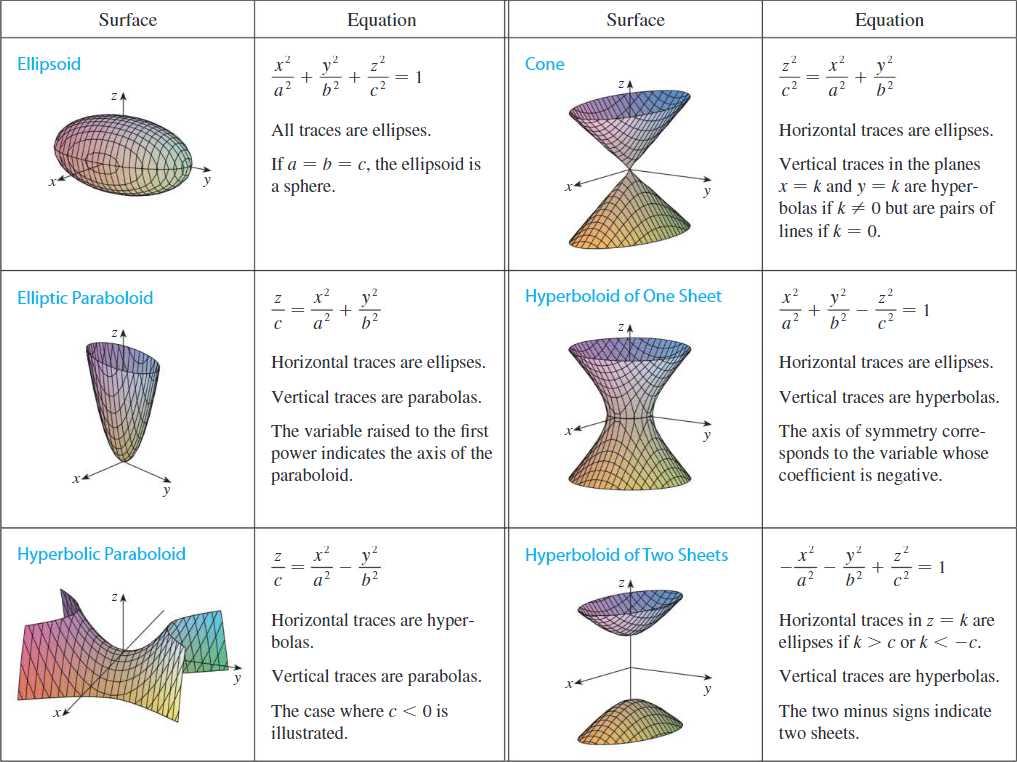
\includegraphics[width=\linewidth]{table13-6.png}
\end{center}